En este capítulo se argumentará la elección de las partes del sistema de adquisición de datos, comparando el hardware seleccionado con las otras opciones evaluadas. También se ilustrarán las dimensiones físicas del soporte y las características de las cámaras empleadas en las pruebas realizadas al paquete.
\section{Características requeridas}
Para poder comprobar el correcto funcionamiento del software, el sistema físico como mínimo debía poseer las siguientes propiedades:
\begin{enumerate}
    \item Capacidad de procesamiento que permita ejecutar el algoritmo de reconocimiento y el de posicionamiento.
    \item Comunicación con el computador donde se desarrolló el paquete.
    \item Cámaras con características similares, preferiblemente iguales para poder realizar el posicionamiento correctamente.
    \item Facilidad de implementación. 
    \item Memoria suficiente que permita guardar el paquete junto a las librerías de las que depende para su funcionamiento.
    \item Una interfaz de usuario accesible.
\end{enumerate}
\section{Estrategias de adquisición de datos}
Se evaluaron 5 estrategias para poder probar las funcionalidades del software diseñado, con el fin de compararlas mediante un gráfico de araña respecto a las cualidades más importantes a tomar en cuenta. 
\\
En todas las estrategias hay una constante y ese es el computador empleado para el diseño del paquete el cual es una Laptop HP 15-dy2xxx con las siguientes especificaciones:
\begin{itemize}
    \item Procesador Quad-core i3-1115G4, con 3.00GHz.  
    \item 8 GB de memoria RAM.
    \item Tarjeta gráfica Intel UHD graphics.
    \item Almacenamiento SSD de 256 GB.
    \item Sistema operativo Linux con la distribución Ubuntu.
    \item Arquitectura de 64 bits.
\end{itemize}
\subsection{Estrategias con módulos StereoPi}
Se evaluaron 3 estrategias distintas que utilizan 3 versiones del módulo StereoPi, las versiones Slim y V1 con el procesador del Raspberry Pi compute module 3+ lite, mientras que la versión 2 del StereoPi con él compute module versión 4 lite. Él compute module actúa como un procesador mientras que el StereoPi funciona como interfaz que recibe las imágenes de las cámaras y se comunica con el computador o con el CM (Compute Module). De igual forma las versiones Slim y V1 se previó usarlas con las cámaras Raspberry Pi V1 (sensor OV5647) y la StereoPi V2 con el sensor IMX219, en la Figura \ref{estrategias_stereopi} se pueden observar el como se conectarían dichas configuraciones, así como también la dirección del flujo de datos.
\begin{figure}[H]
     \centering
     \begin{subfigure}[b]{0.4\textwidth}
        \centering
        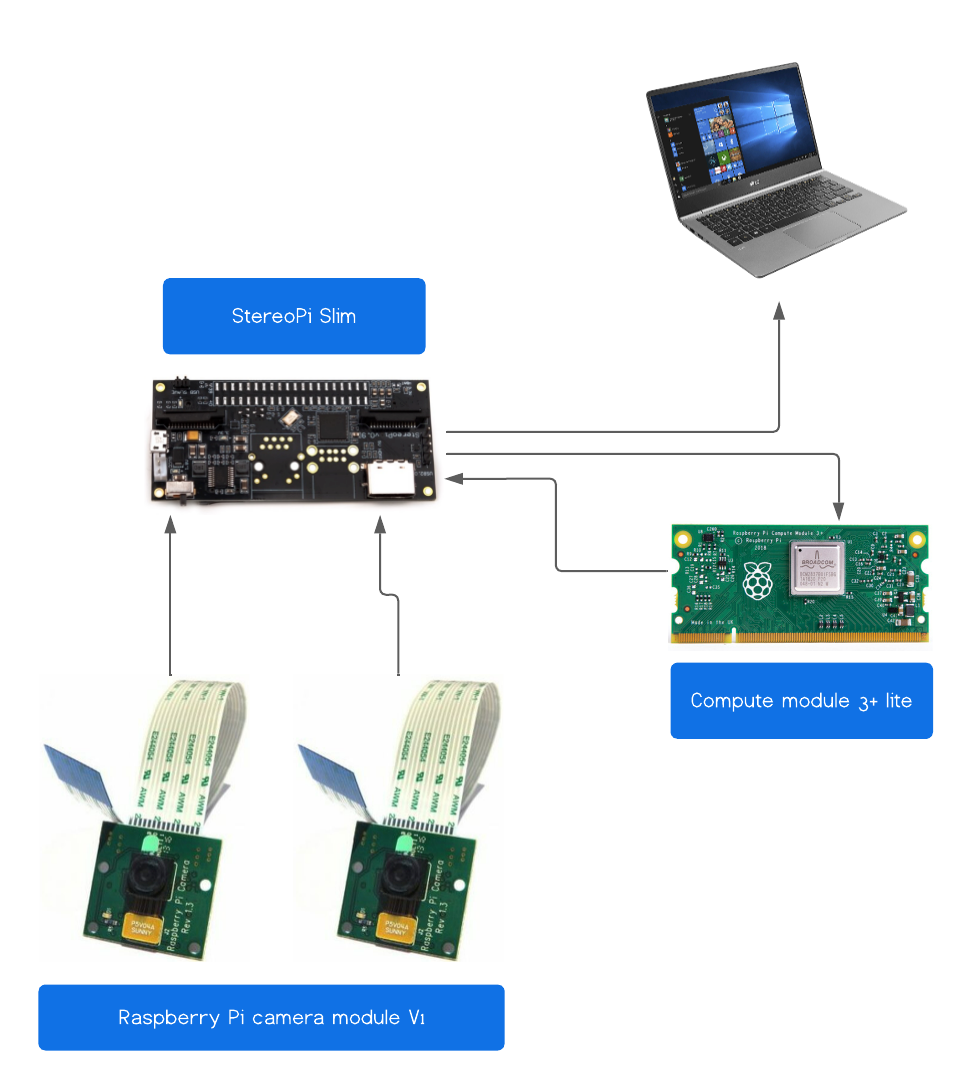
\includegraphics[scale=0.4]{Recursos/estrategia_stereopi_slim.png}
        \caption{Estrategia StereoPi Slim}
        \label{estrategia_slim}
     \end{subfigure}
     \hfill
     \begin{subfigure}[b]{0.4\textwidth}
         \centering
        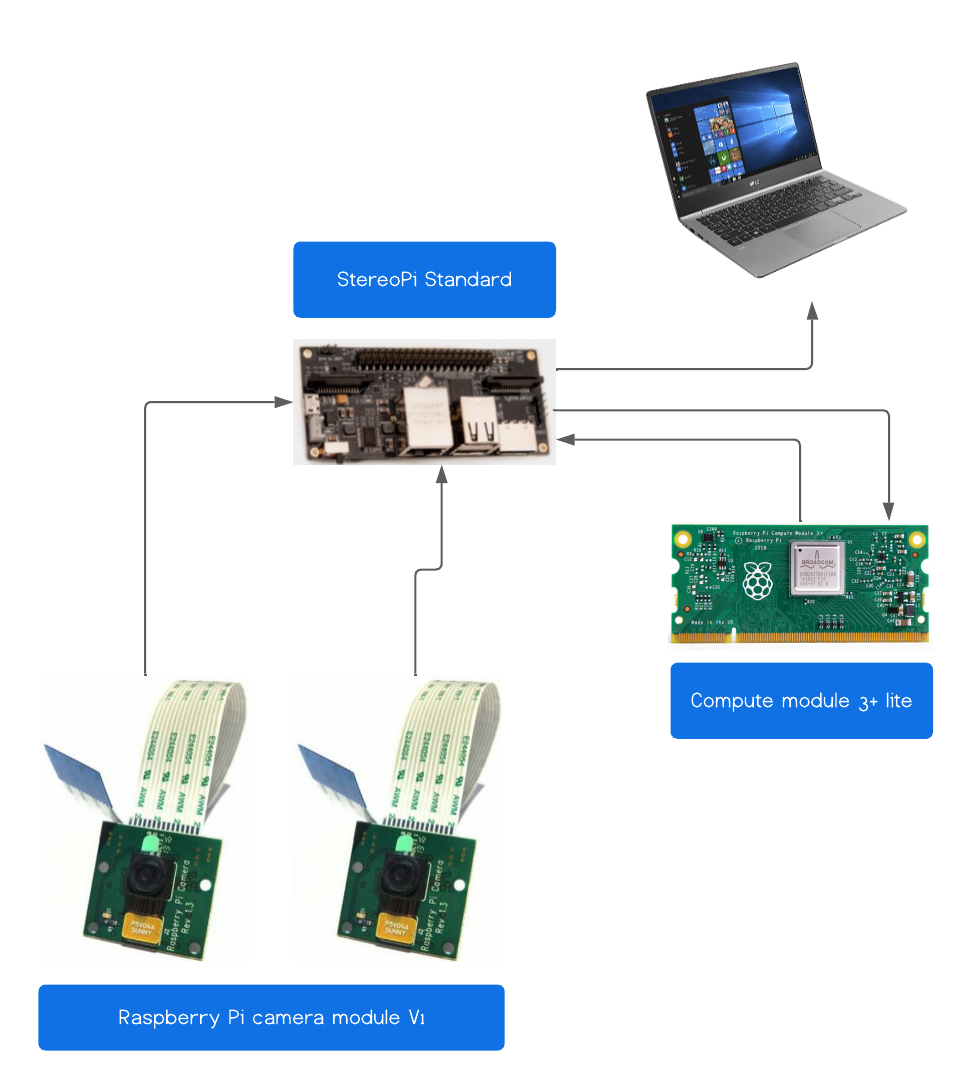
\includegraphics[scale=0.4]{Recursos/estrategia_stereo_pi_standard.png}
        \caption{Estrategia StereoPi V1}
        \label{estrategia_v1}
     \end{subfigure}
     \hfill
     \begin{subfigure}[b]{0.4\textwidth}
         \centering
        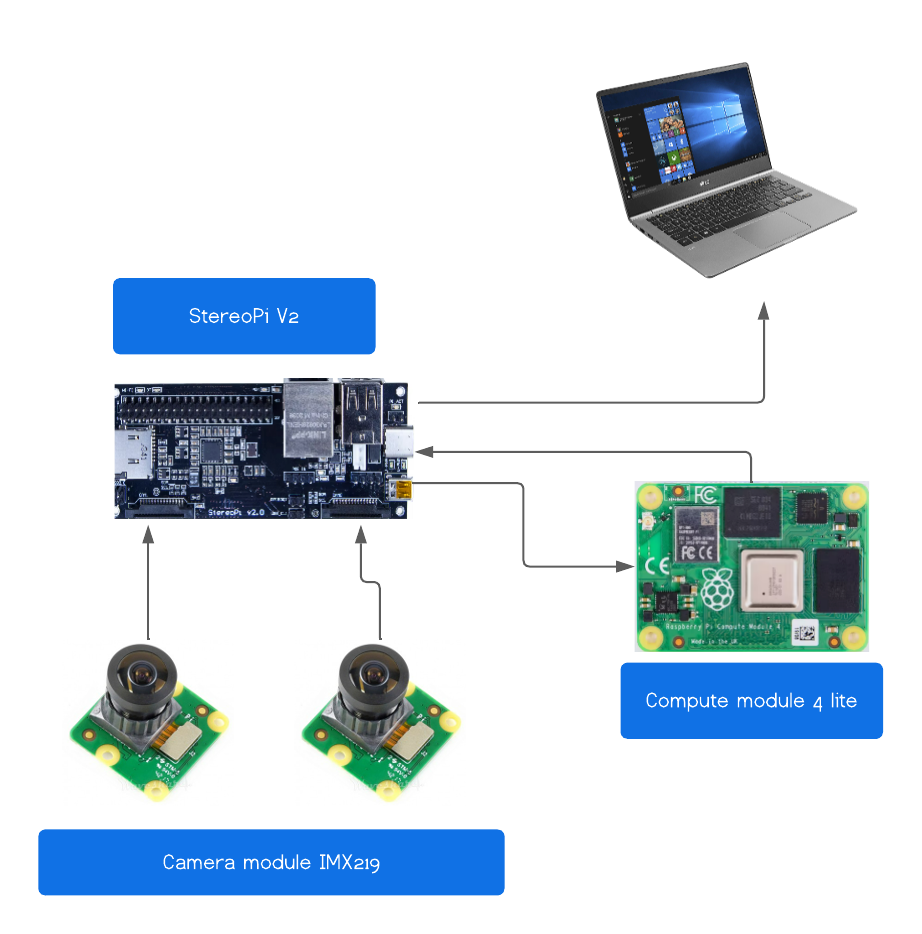
\includegraphics[scale=0.4]{Recursos/estrategia_stereopi_v2.png}
        \caption{Estrategia StereoPi V2}
        \label{estrategia_v2}
     \end{subfigure}
     \hfill
\caption{Configuraciones basadas en módulo StereoPi}
\label{estrategias_stereopi}
\end{figure}
En la Tabla \ref{comparacion_stereopi} se presenta una comparación entre las características más importantes de las 3 estrategias.
\begin{table}[H]
\centering
\caption{Especificaciones de estrategias StereoPi}
\label{comparacion_stereopi}
\begin{tabular}{l|ccc|}
\cline{2-4}
 & \multicolumn{3}{c|}{Estrategias} \\ \hline
\multicolumn{1}{|l|}{Características} & \multicolumn{1}{c|}{StereoPi Slim} & \multicolumn{1}{c|}{StereoPi V1} & StereoPi V2 \\ \hline
\multicolumn{1}{|l|}{Wifi} & \multicolumn{1}{c|}{No} & \multicolumn{1}{c|}{No} & Si \\ \hline
\multicolumn{1}{|l|}{Bluetooth} & \multicolumn{1}{c|}{No} & \multicolumn{1}{c|}{No} & Si \\ \hline
\multicolumn{1}{|p{2.5cm}|}{CPU} & \multicolumn{1}{p{2.5cm}|}{ARM Cortex-A53 64-bit @ 1.2GHz} & \multicolumn{1}{p{2.5cm}|}{ARM Cortex-A53 64-bit @ 1.2GHz} &\multicolumn{1}{p{2.5cm}|}{ARM Cortex-A72 64-bit @ 1.5GHz} \\ \hline
\multicolumn{1}{|p{2.5cm}|}{RAM} & \multicolumn{1}{p{2.5cm}|}{1GB LPDDR2 SDRAM} & \multicolumn{1}{p{2.5cm}|}{1GB LPDDR2 SDRAM} & \multicolumn{1}{p{2.5cm}|}{2GB LPDDR4-3200 SDRAM} \\ \hline
\multicolumn{1}{|p{3cm}|}{Almacenamiento} & \multicolumn{1}{p{2.5cm}|}{micro SD} & \multicolumn{1}{p{2.5cm}|}{micro SD} & \multicolumn{1}{p{2.5cm}|}{micro SD } \\ \hline
\multicolumn{1}{|p{2.5cm}|}{Sistema operativo} & \multicolumn{1}{p{2.5cm}|}{Raspbian} & \multicolumn{1}{p{2.5cm}|}{Raspbian} & \multicolumn{1}{p{2.5cm}|}{Raspbian} \\ \hline
\multicolumn{1}{|p{2.5cm}|}{Ethernet} & \multicolumn{1}{c|}{No} & \multicolumn{1}{c|}{Si} & Si \\ \hline
\multicolumn{1}{|p{2.5cm}|}{HDMI} & \multicolumn{1}{c|}{Si} & \multicolumn{1}{c|}{Si} & Si \\ \hline
\multicolumn{1}{|p{2.5cm}|}{USB} & \multicolumn{1}{c|}{1 x micro} & \multicolumn{1}{c|}{2 x Tipo A, 1 x micro} & 2 x Tipo A, 1 x Tipo C \\ \hline
\multicolumn{1}{|p{2.5cm}|}{Video} & \multicolumn{1}{p{2.5cm}|}{1080p30, 720p60 y 640x480p90} & \multicolumn{1}{p{2.5cm}|}{1080p30, 720p60 y 640x480p90} & \multicolumn{1}{p{2.5cm}|}{1080p30, 720p60 y 640x480p90} \\ \hline
\multicolumn{1}{|p{2.5cm}|}{Resolución de cámara} & \multicolumn{1}{c|}{5 MP} & \multicolumn{1}{p{2.5cm}|}{5 MP} & 8 MP \\ \hline
\end{tabular}
\end{table}
\subsection{Estrategia con Jetson Nano B01 y módulo IMX219-83}
Como su nombre lo indica esta emplea un módulo Jetson Nano B01 cuyas cualidades relevantes son:
\begin{itemize}
    \item \textbf{GPU:} 128 núcleos con la arquitectura Maxwell de NVIDIA.
    \item \textbf{CPU:} ARM 57 Quad-core.
    \item \textbf{Memoria RAM:} 4 GB LPDDR4.
    \item \textbf{Entradas/salidas:} Ethernet, 4 USB 3.0, micro USB, HDMI, UART, I2C, SPI, 2 puertos MIPI-CSI (conectores de cámaras).
\end{itemize}
El módulo IMX219-83 es un integrado que contiene dos cámaras, acompañadas del chip ICM20948, sin embargo a continuación se listarán las características únicamente del elemento estéreo:
\begin{itemize}
    \item \textbf{Megapíxeles:} 8 MP.
    \item \textbf{Resolución:} 3280 × 2464 px (por cámara).
    \item \textbf{FOV:} 83/73/50 grados (diagonal/horizontal/vertical).
    \item \textbf{Distancia focal:} 2.6 mm
    \item \textbf{Línea base:} 60 mm.
\end{itemize}
En la Figura \ref{estrategia_jetson} se puede observar un diagrama que representa como se aplicaría esta estrategia.
\begin{figure}[H]
    \centering
    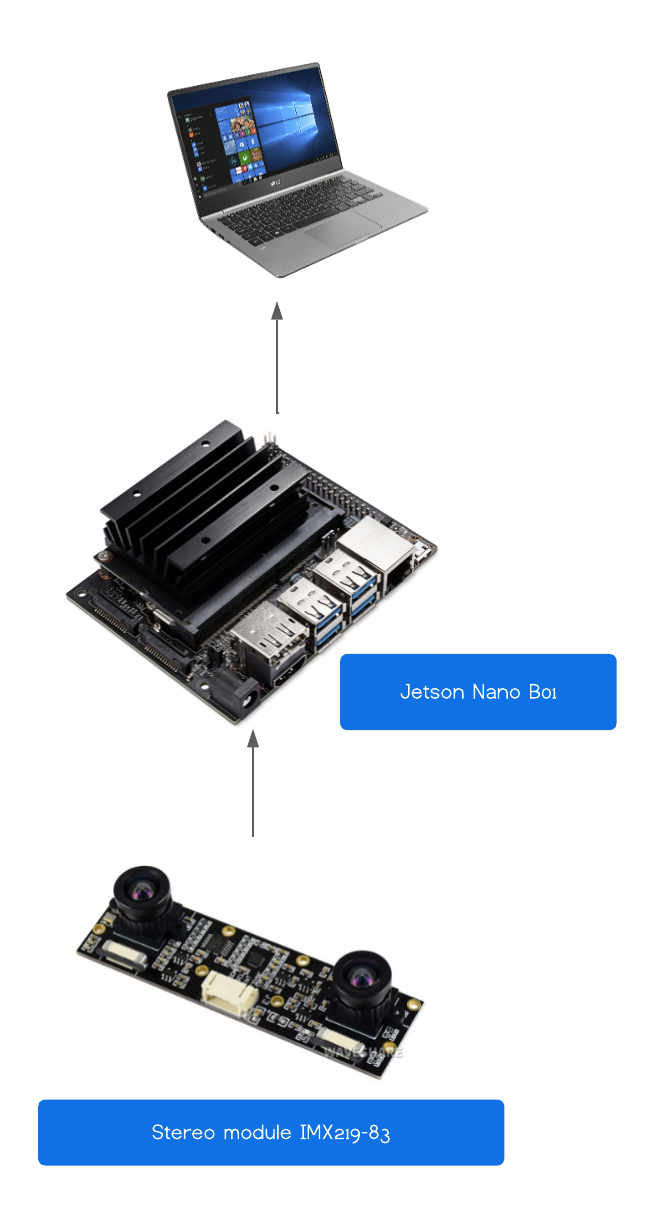
\includegraphics[scale=0.5]{Recursos/estrategia_jestson_nano.png}
    \caption{Estrategia con Jetson Nano B01}
    \label{estrategia_jetson}
\end{figure}
\subsection{Estrategia con dos teléfonos}
Usando las cámaras de dos teléfonos a los cuales el autor tiene acceso y transmitiendo lo que observa cada cámara a un servidor local para captar ambas imágenes mediante el computador el cual realizara todo el procesamiento, es posible crear un sistema estéreo como el de la Figura \ref{estrategia_phone}.
\begin{figure}[H]
    \centering
    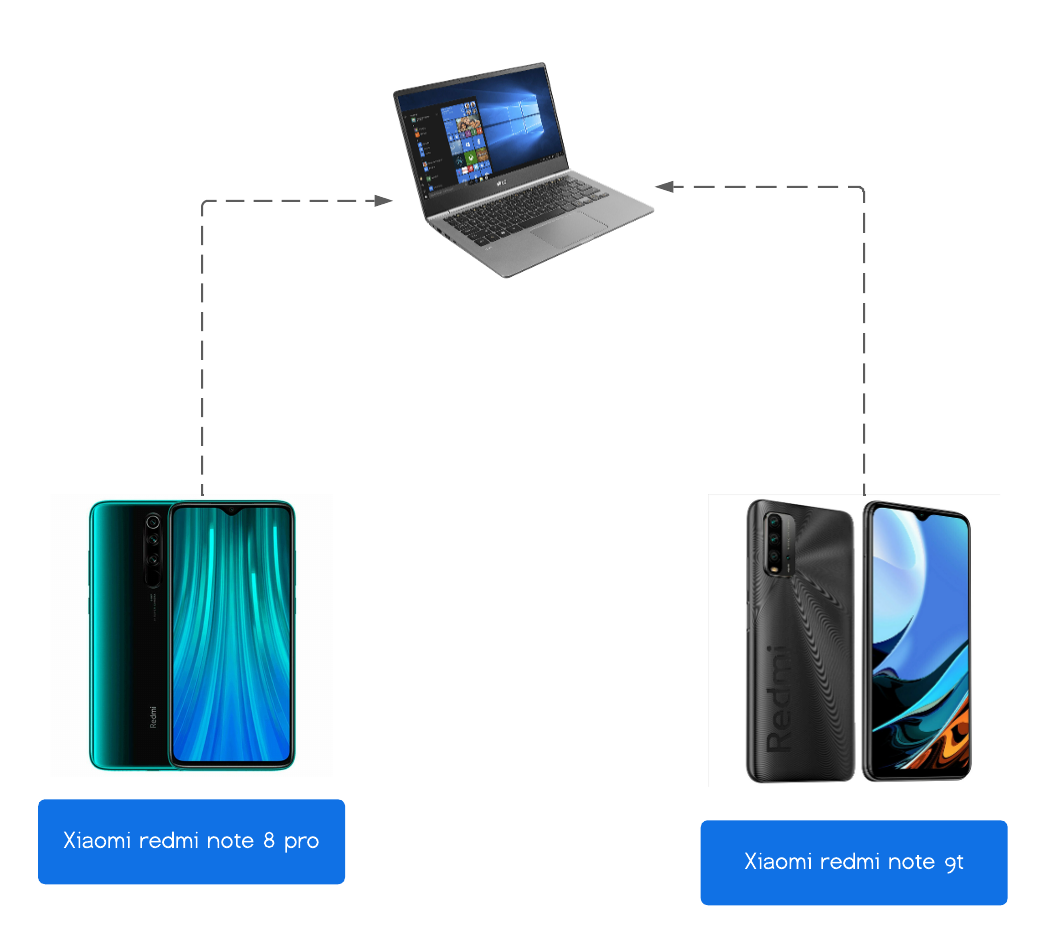
\includegraphics[scale=0.5]{Recursos/estrategia_telefonos.png}
    \caption{Estrategia con teléfonos}
    \label{estrategia_phone}
\end{figure}
Los teléfonos presentes en la Figura \ref{estrategia_phone} poseen las siguientes características:
\begin{itemize}
    \item Xiaomi redmi note 8 pro: sus dimensiones son 161.3 x 76.4 x 8.8 mm, posee 5 cámaras, con una resolución máxima de 64 MP.
    \item Xiaomi redmi 9T: sus dimensiones son 162.3 x 77.3 x 9.6 mm, posee 5 cámaras, con una resolución máxima de 48 MP.
\end{itemize}
\subsection{Elección de estrategia}
\begin{figure}[H]
    \centering
    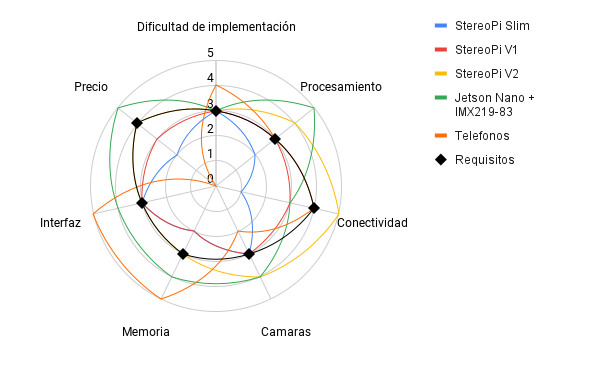
\includegraphics[scale=0.5]{Recursos/spyder_chart.png}
    \caption{Comparación de estrategias}
    \label{spyder_chart}
\end{figure}
En la Figura \ref{spyder_chart} se observan 7 parámetros que sintetizan las características requeridas expuestas anteriormente, por lo que a continuación se explicaran las razones de las puntuaciones obtenidas.
\begin{itemize}
    \item \textbf{Dificultad de implementación:} este parámetro permite medir que tan sencillo seria integrar todos los elementos de la estrategia, con el objetivo de poner en funcionamiento el sistema y probar las herramientas del paquete, en este caso es conveniente que sea sencillo, para así poder concentrar el trabajo en el paquete y no en la implementación física, como se puede observar en la Figura \ref{spyder_chart} el más complicado de implementar es el que emplea teléfonos, puesto que requiere diseñar y construir una estructura que pueda soportar ambos teléfonos y que a su vez ubique perfectamente los centros ópticos en una disposición paralela.
    \item \textbf{Procesamiento:} relacionado con la capacidad del CPU y la GPU en el caso de la Jetson Nano, ya que esta permite ejecutar modelos de aprendizaje automático de forma más eficiente. Como se puede observar en la Figura \ref{spyder_chart} al menos 4 de 5 son capaces de cumplir con este parámetro.
    \item \textbf{Conectividad:} este se relaciona con las formas de poder conectarse con el computador donde se esta desarrollando el paquete y dado que el StereoPi V2 posee conexión mediante wifi es posible probar como funciona el paquete cuando las imágenes son enviadas de forma remota al igual que con dos dispositivos móviles.
    \item \textbf{Cámaras:} esto va ligado tanto a la calidad de la imagen y el vídeo, como al hecho de que ambas cámaras tengan características similares, razón por la cual la opción de los teléfonos se ve fuertemente penalizada, porque si bien es cierto que es posible realizar estéreo con cámaras distintas y sin conocer los parámetros, también es correcto decir que calibrar los parámetros intrínsecos e extrínsecos de teléfonos distintos puede llevar a un mayor error al momento de hallar el mapa de disparidad.
    \item \textbf{Memoria:} el método elegido debe ser capaz de poder almacenar las librerías que se utilizan en el paquete.
    \item \textbf{Interfaz:} a mayor puntación será más sencillo implementar el paquete, razón del porqué la opción de los teléfonos tiene el valor máximo, ya que; de emplearla el procesamiento es realizado mediante el computador, por lo que no sería necesario diseñar una app móvil, ya que existen aplicaciones como IP webcam que permiten crear un servidor local y transmitir vídeo a este.
    \item \textbf{Precio:} un factor tan relevante como los anteriores al momento de dimensionar cualquier sistema.
\end{itemize}
Como se puede observar en la Figura \ref{spyder_chart} el método con teléfonos tiene un coste 0, debido a que ya se poseen ambos dispositivos e incluso el resto de sus puntuaciones son bastante buenas a excepción del esfuerzo que implica construir la estructura de soporte; sin embargo, dicha opción tiene un problema que impediría el correcto funcionamiento del sistema y esa es su puntuación en las cámaras, por otro lado si bien el módulo de desarrollo de NVIDIA cumple excepcionalmente en casi todo, su costo es muy elevado y no posee comunicación inalámbrica por lo que para poder comprobar el funcionamiento de todo el paquete sería necesario agregar un módulo de wifi aparte, lo que elevaría aún más el costo final. En el caso del StereoPi V1 posee el mismo problema de conectividad y puede que su memoria sea insuficiente e incluso la capacidad de procesamiento queda ajustada. Por estos motivos se seleccionó la estrategia StereoPi V2.  
\subsection{Implementación del sistema de adquisición de datos}
Para poder armar la estrategia seleccionada no solo fueron necesarios los elementos ya mencionados, debido a que el soporte físico sobre el que se sustentaría el StereoPi y el Compute Module 4 lite era un componente de vital importancia para poder mantener el conjunto de cámaras en una posición fija, a tal efecto se empleó una montura como el que utilizan las cámaras GoPro, (Ver Figura \ref{gopro_support}) la cual está compuesta de 3 partes una arandela, 1 tornillo para ajustar y un trípode.
\begin{figure}[H]
    \centering
    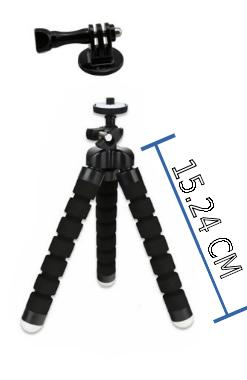
\includegraphics[scale=0.5]{Recursos/go_pro_support.jpg}
    \caption{Montura del sistema tipo GoPro}
    \label{gopro_support}
\end{figure}
\subsubsection{Ensamblado}
Se siguieron los siguientes pasos para armar el sistema:
\begin{enumerate}
    \item Se posicionaron el módulo StereoPi V2 y el CM4 lite como en la Figura \ref{connect_cm4} y posteriormente se conectaron.
    \begin{figure}[H]
        \centering
        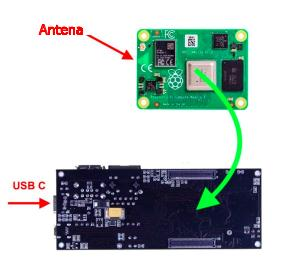
\includegraphics{Recursos/cm4_connect.jpg}
        \caption{Conexión entre CM4 lite y StereoPi V2}
        \label{connect_cm4}
    \end{figure}
    \item Se insertó una tarjeta SD de 32 GB en el StereoPi V2, aunque para permitir el acceso a dicha memoria con el fin de programar, se le colocaron 3 jumpers al StereoPi V2 que cortocircuitan los pines RPIBOOT, USB slave y power switch, los cuales se localizan como en la Figura \ref{stereoPi_IO}
    \begin{figure}[H]
        \centering
        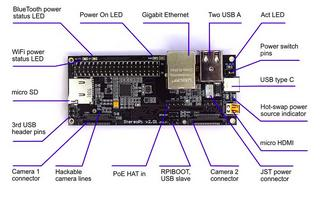
\includegraphics{Recursos/stereoPi_IO.jpg}
        \caption{Entradas y salidas del StereoPi V2. Imagen de \cite{stereopi_quickstart_guide}}
        \label{stereoPi_IO}
    \end{figure}
    \item Con uno de los moldes impresos en acrílico, 4 tuercas y 4 espaciadores de 10 mm se armó la base de las cámaras como en la Figura \ref{camera_base}.
    \begin{figure}[H]
        \centering
        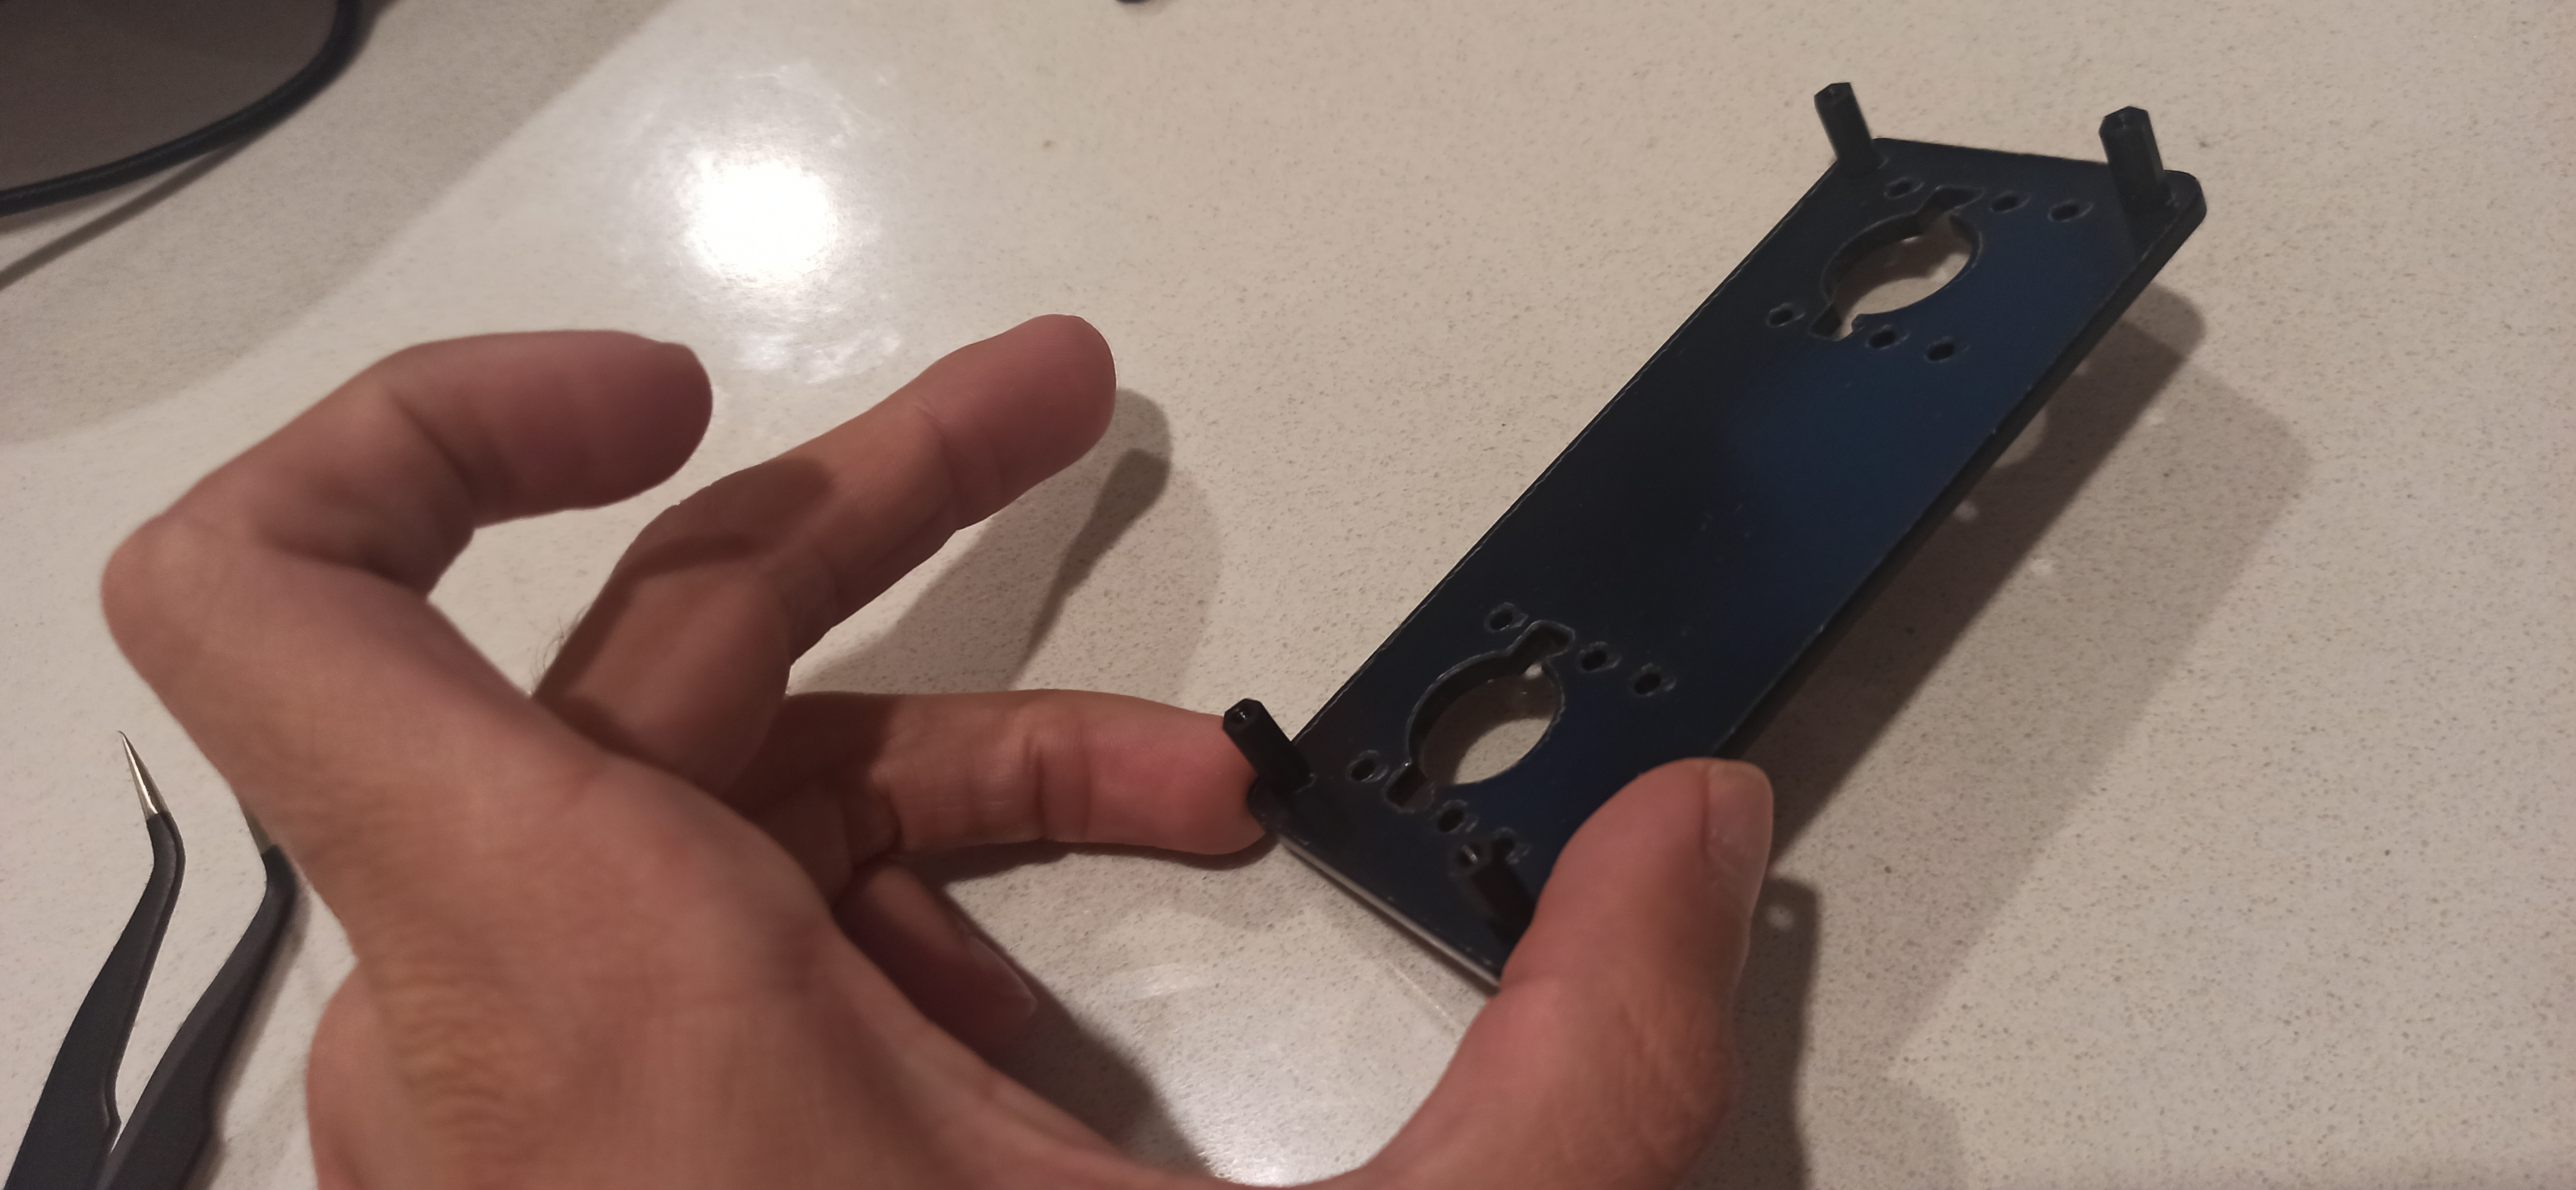
\includegraphics[scale=0.05]{Recursos/camera_base.jpg}
        \caption{Base de las cámaras IMX219 instalada}
        \label{camera_base}
    \end{figure}
    \item A la base armada en el paso previo se le acoplaron 2 cámaras IMX219 con 8 tornillos y 8 tuercas (ver Figura \ref{cameras_installed}). Las cámaras cuentan con una resolución de 8 MP, pueden captar imágenes de hasta 3280 x 2464 píxeles, transmitir vídeo con una resolución y cuadros por segundo de 1080p30, 720p60 y 640x480p90, son compatibles con interfaces CSI (Camera Serial Interface), poseen un Field of view (FOV) de 160$^0$, cuentan con un lente con una apertura de 2.35 y una distancia focal de 3.15 mm.
    \begin{figure}[H]
        \centering
        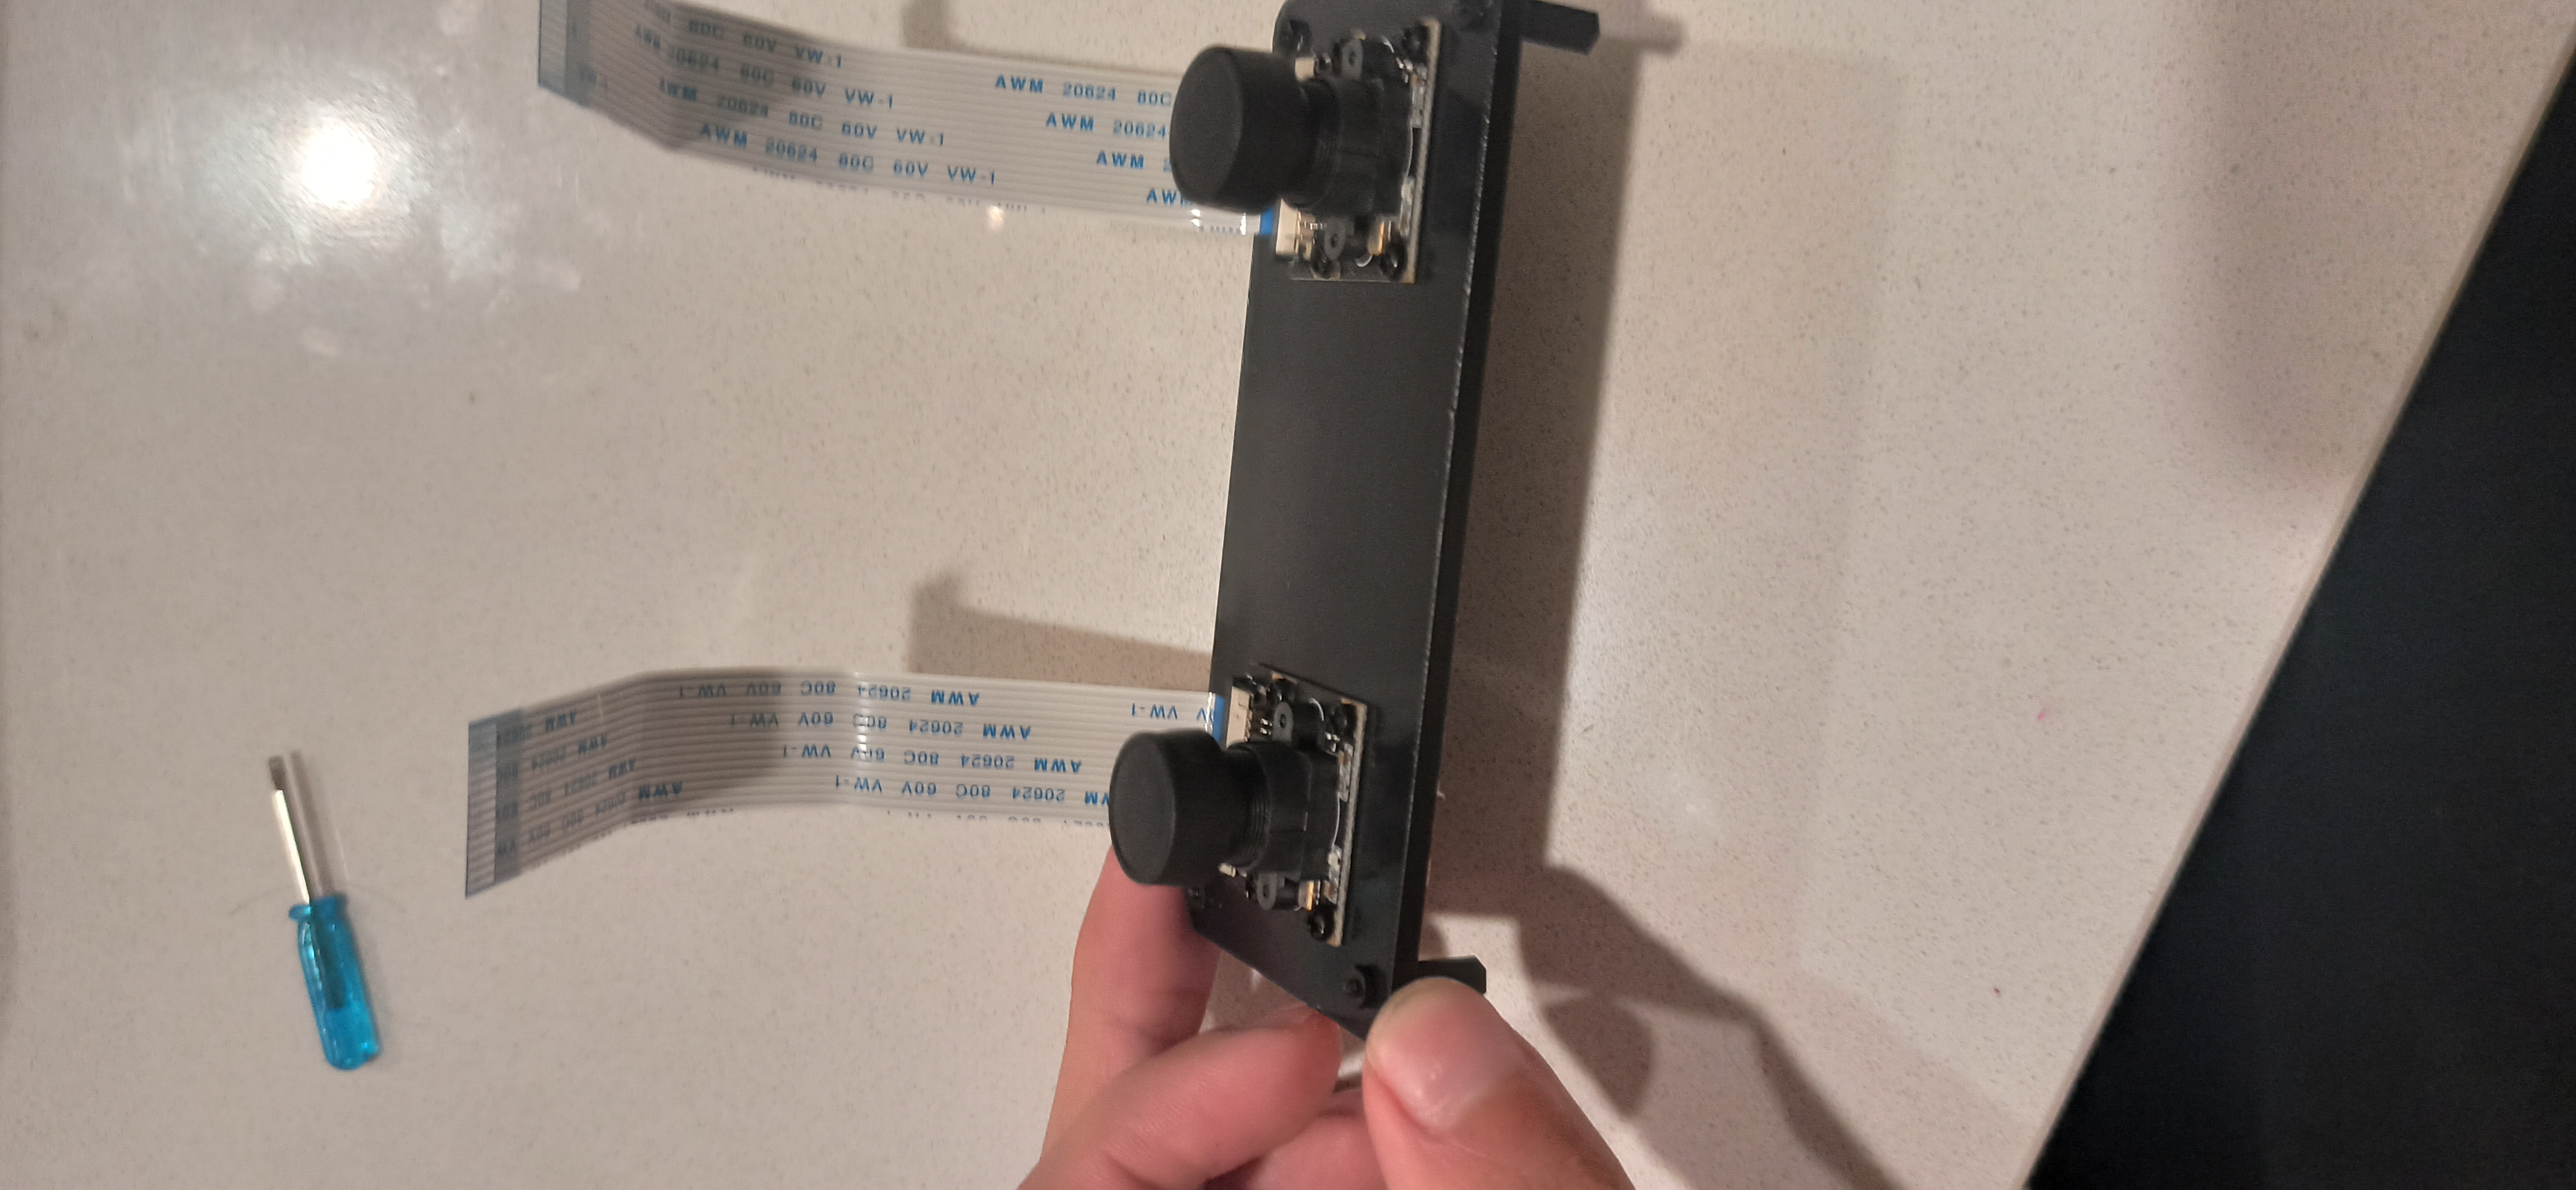
\includegraphics[scale=0.05]{Recursos/camera_installed.jpg}
        \caption{Módulos IMX219 instalados}
        \label{cameras_installed}
    \end{figure}
    \item Se conectaron las cámaras al módulo estéreo y se ensambló el último a la base de las cámaras con 4 espaciadores de 20 mm como en la Figura \ref{module_installed}.
    \begin{figure}[H]
        \centering
        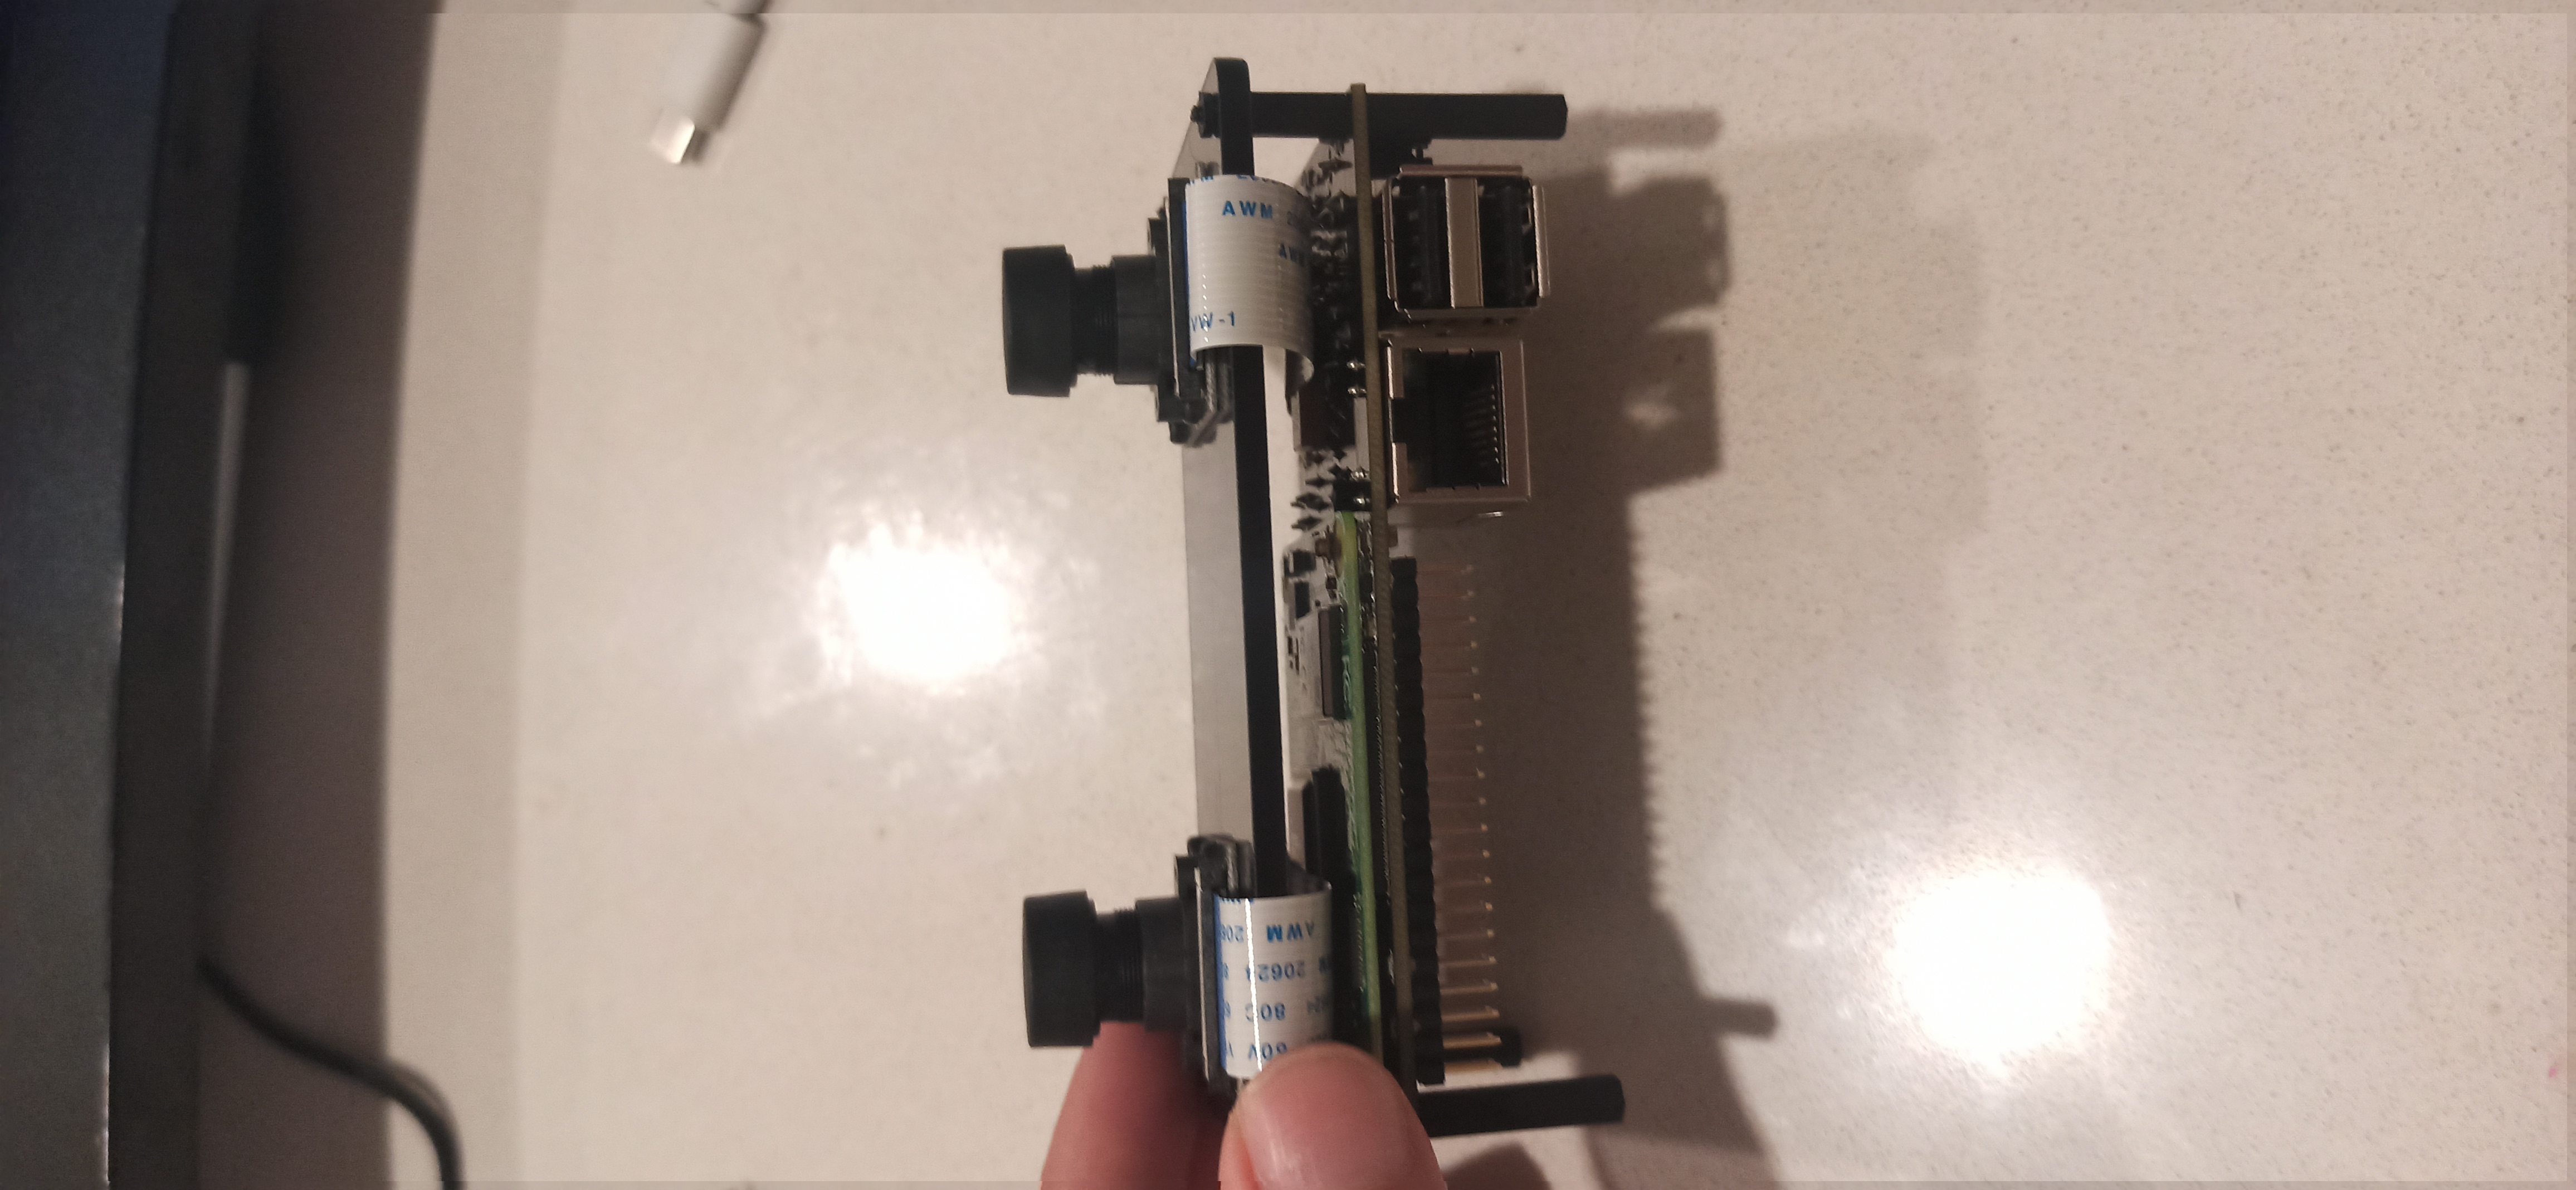
\includegraphics[scale=0.05]{Recursos/module_installed.jpg}
        \caption{IMX219 acoplados al StereoPi V2 y compute module 4 lite}
        \label{module_installed}
    \end{figure}
    \item Para fijar todas las piezas y poder conectar la estructura con la montura de la GoPro se conectó la otra pieza de acrílico con 4 tornillos al igual que en la Figura \ref{two_acrilics}.
    \begin{figure}[H]
        \centering
        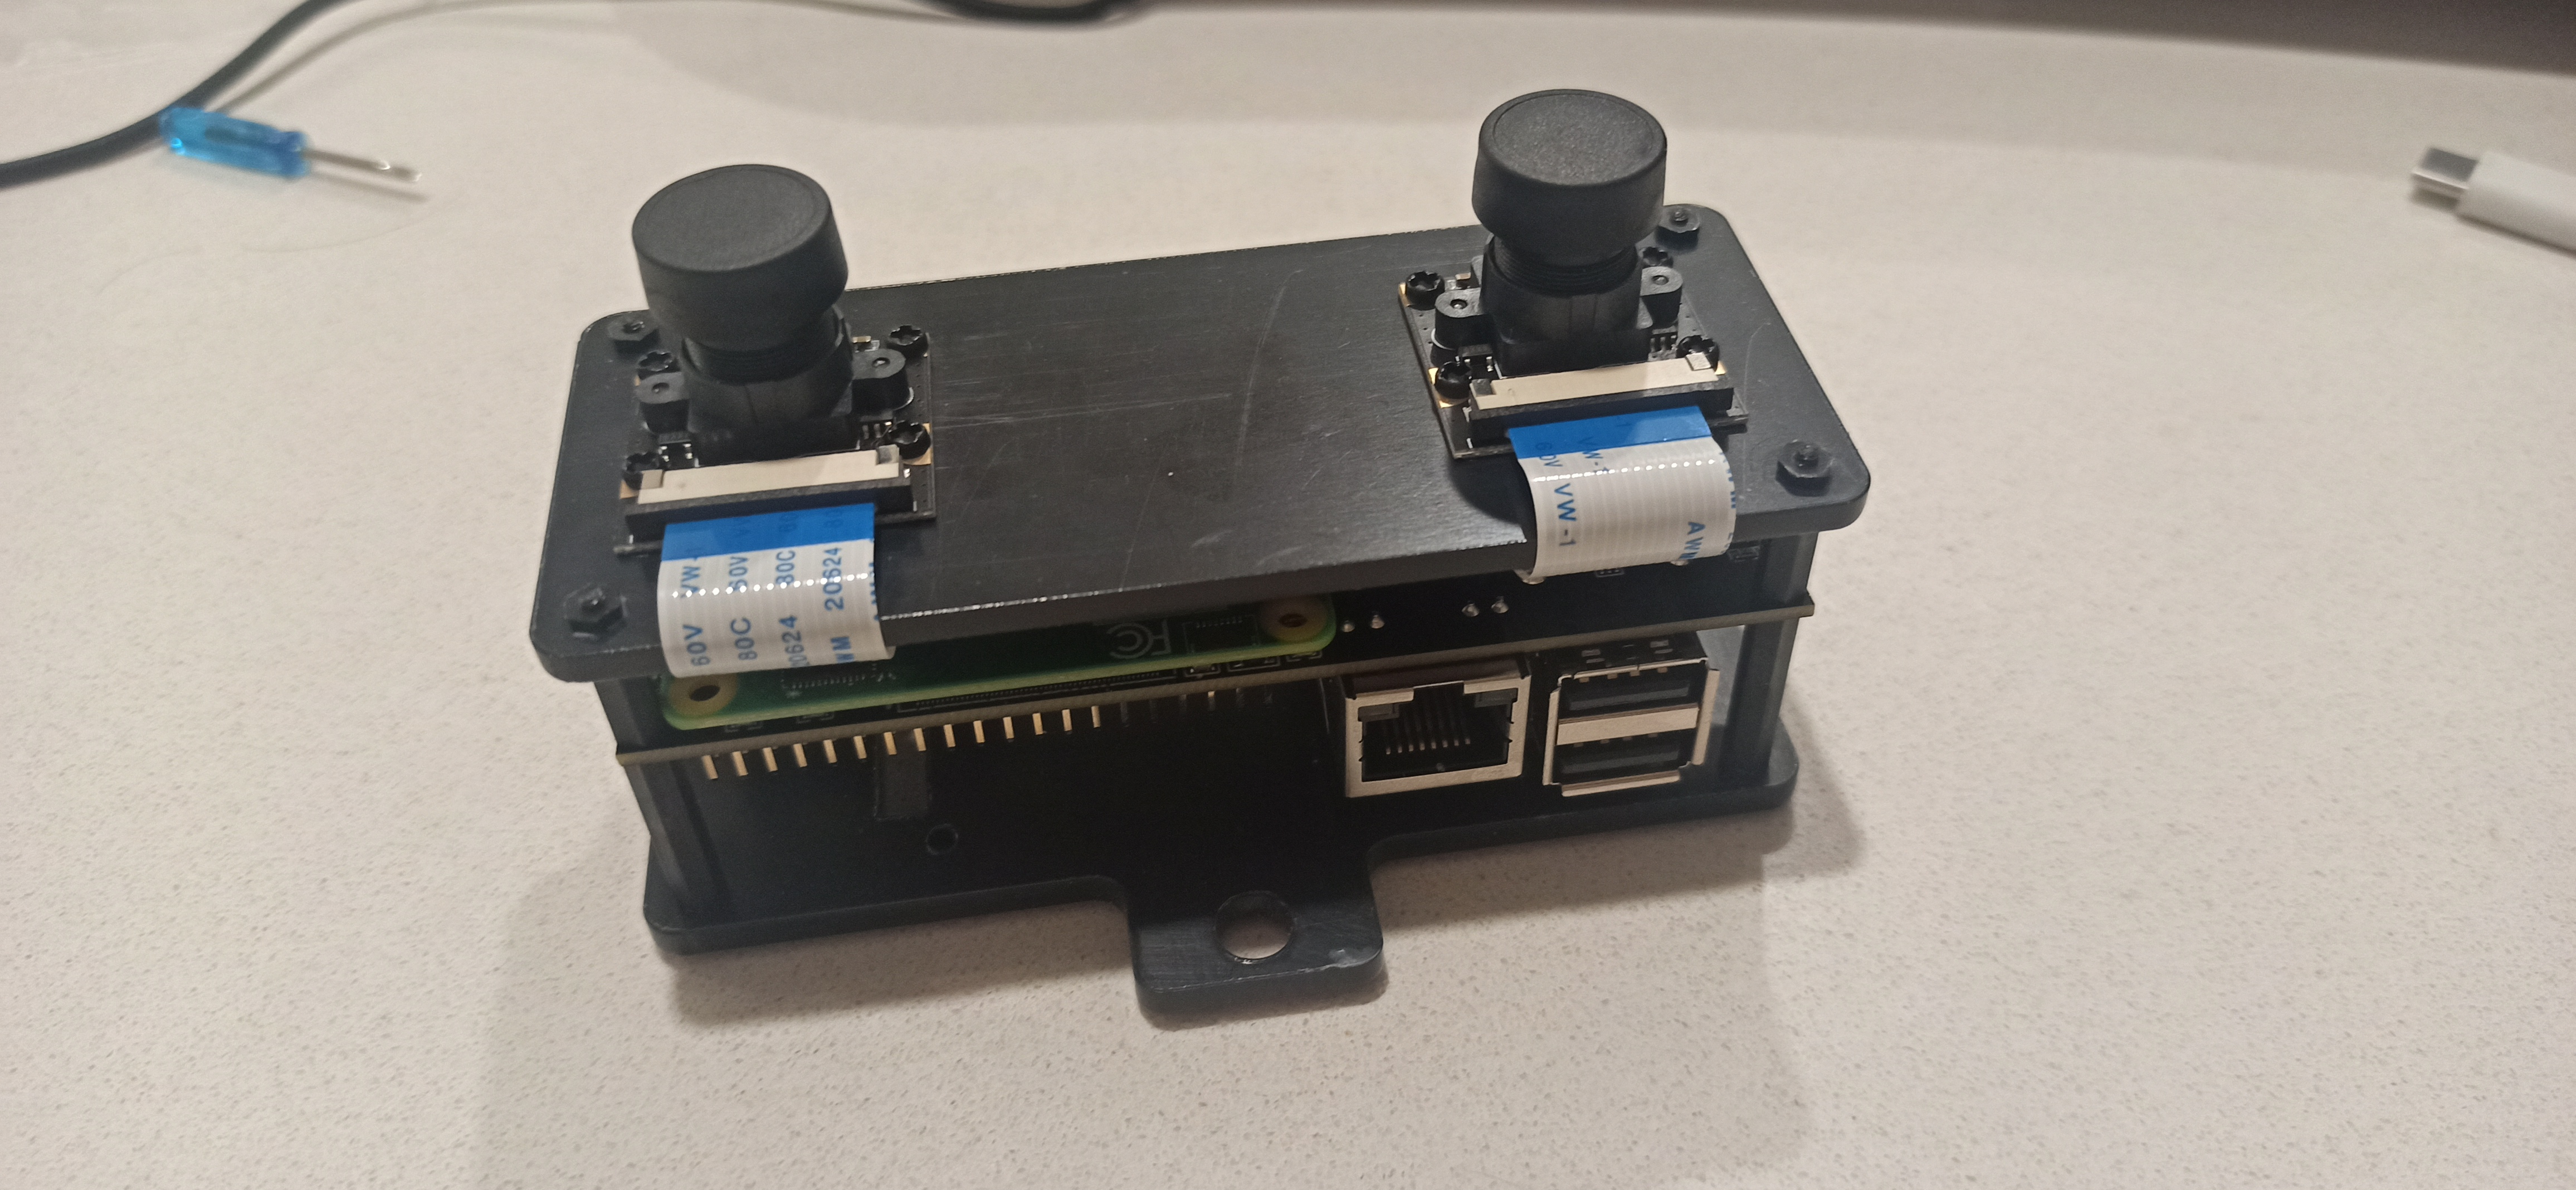
\includegraphics[scale=0.05]{Recursos/two_pastic_installed.jpg}
        \caption{Estructura de adquisición de datos sin montura}
        \label{two_acrilics}
    \end{figure}
    \item Se conectó la estructura con la montura de la GoPro (ver Figura \ref{implemented_stereo_pi}).
    \begin{figure}[H]
        \centering
        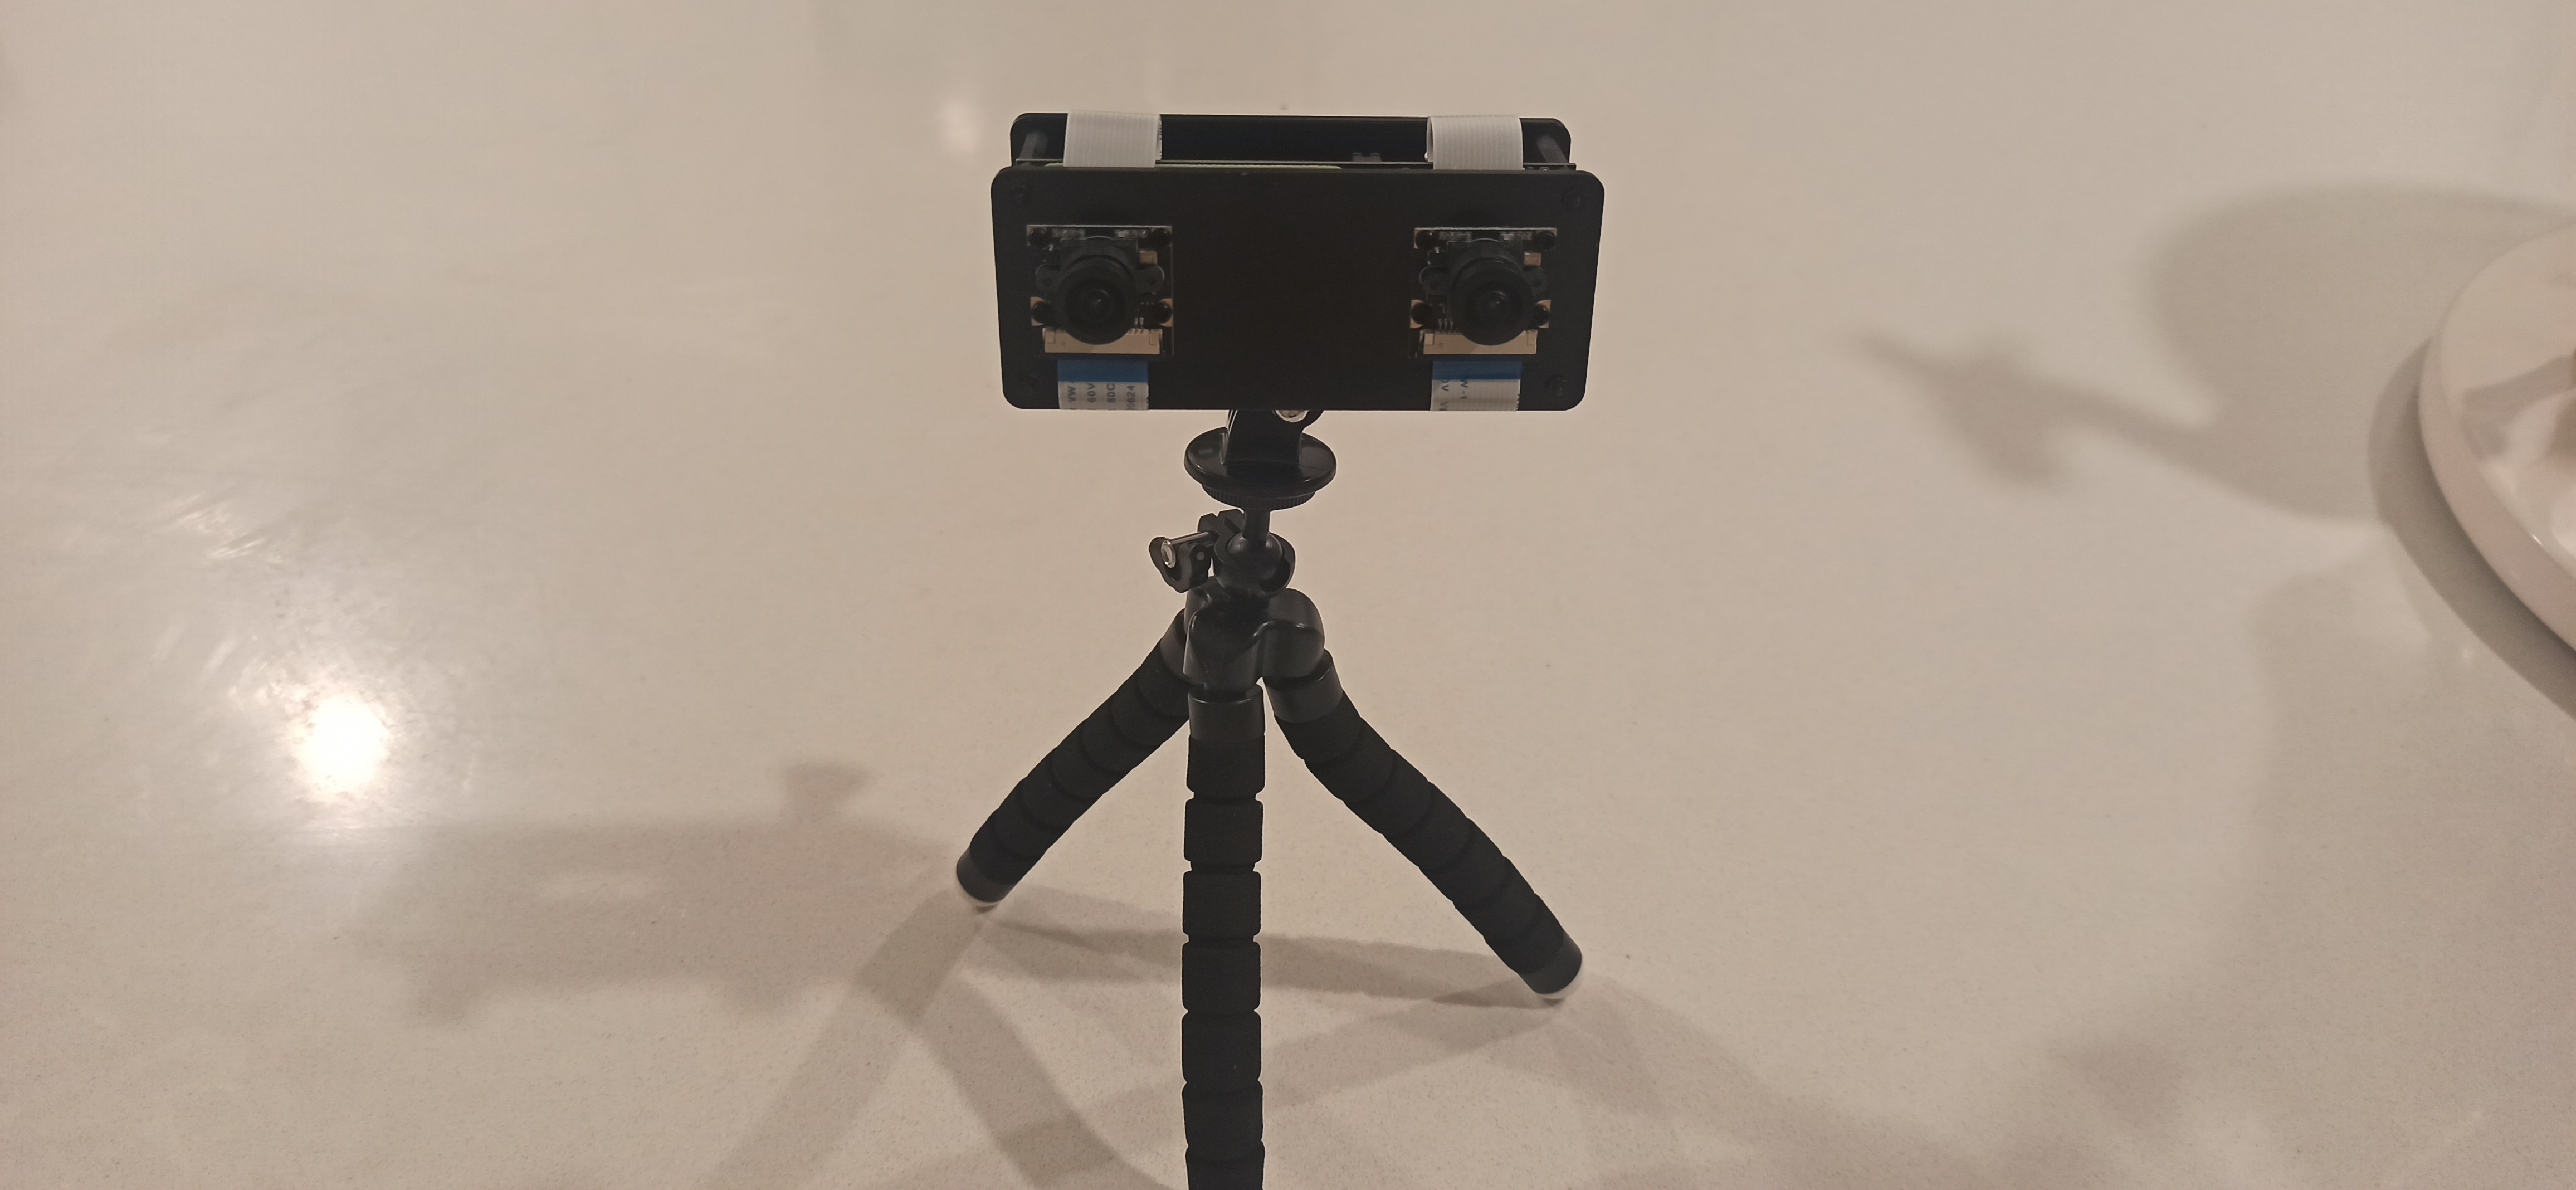
\includegraphics[scale=0.05]{Recursos/implemented_stereopiv2.jpg}
        \caption{Implementación del sistema}
        \label{implemented_stereo_pi}
    \end{figure}
    \item Adicionalmente se le anexó una antena al CM4 lite para comprobar las funciones inalámbricas del paquete.
\end{enumerate}
En la tabla \ref{BOM} se listan los materiales empleados para la implementación del sistema.
\begin{table}[H]
\centering
\caption{Lista de materiales}
\label{BOM}
\begin{tabular}{|c|c|c|}
\hline
Cantidad & Ítem                           & Características             \\ \hline
1        & Módulo StereoPi                & Versión 2.02                \\ \hline
1        & Memoria SD                     & 32 GB                       \\ \hline
1        & Raspberry Pi Compute Module 4  & Versión lite                \\ \hline
2        & Cámara IMX-219                 & FOV 160$^0$                \\ \hline
2        & Pieza de acrílico              & -                           \\ \hline
3        & Jumper para cortocircuitar PCB & -                           \\ \hline
1        & Montura de GoPro               & 15.24 cm                    \\ \hline
4        & Espaciador                     & 20 mm                       \\ \hline
4        & Espaciador                     & 10 mm                       \\ \hline
12       & Tuercas                        & plástico                    \\ \hline
12       & Tornillos                      & Tipo cruz                   \\ \hline
1        & Antena                         & -                           \\ \hline
1        & USB                            & Tipo C                      \\ \hline
\end{tabular}
\end{table}